\subsection{Эллипс}

{\bfseries \term{Эллипс}}~--- плоская замкнутая кривая, сумма расстояний от любой точки которой до двух фиксированных точек, называемых фокусами, постоянна.
\begin{equation}
	|F_1 M| + |F_2 M|=\const
\end{equation}
\change{\imp{Центром} эллипса называется середина отрезка, соединяющего его фокусы.}

\begin{minipage}{0.5\tw}
	\change{\imp{Большая ось} эллипса~--- прямая, проходящая через фокусы эллипса; \imp{малая ось}~--- прямая ей перпендикулярная и проходящая через центр эллипса.}
	
	\change{
	Главные отрезки эллипса: \term{большая полуось} ($a$)~--- расстояние от центра эллипса до его пересечения с большой осью; \term{малая полуось} ($b$) определяется дословно также, заменив большую ось на малую; \term{фокальное расстояние} ($c$)~--- расстояние от центра эллипса до одного из фокусов, что тоже самое, половина расстояния между фокусами.
	}
\end{minipage}
\begin{minipage}{0.5\tw}
	\begin{flushright}
		\vspace{-.5pc}
		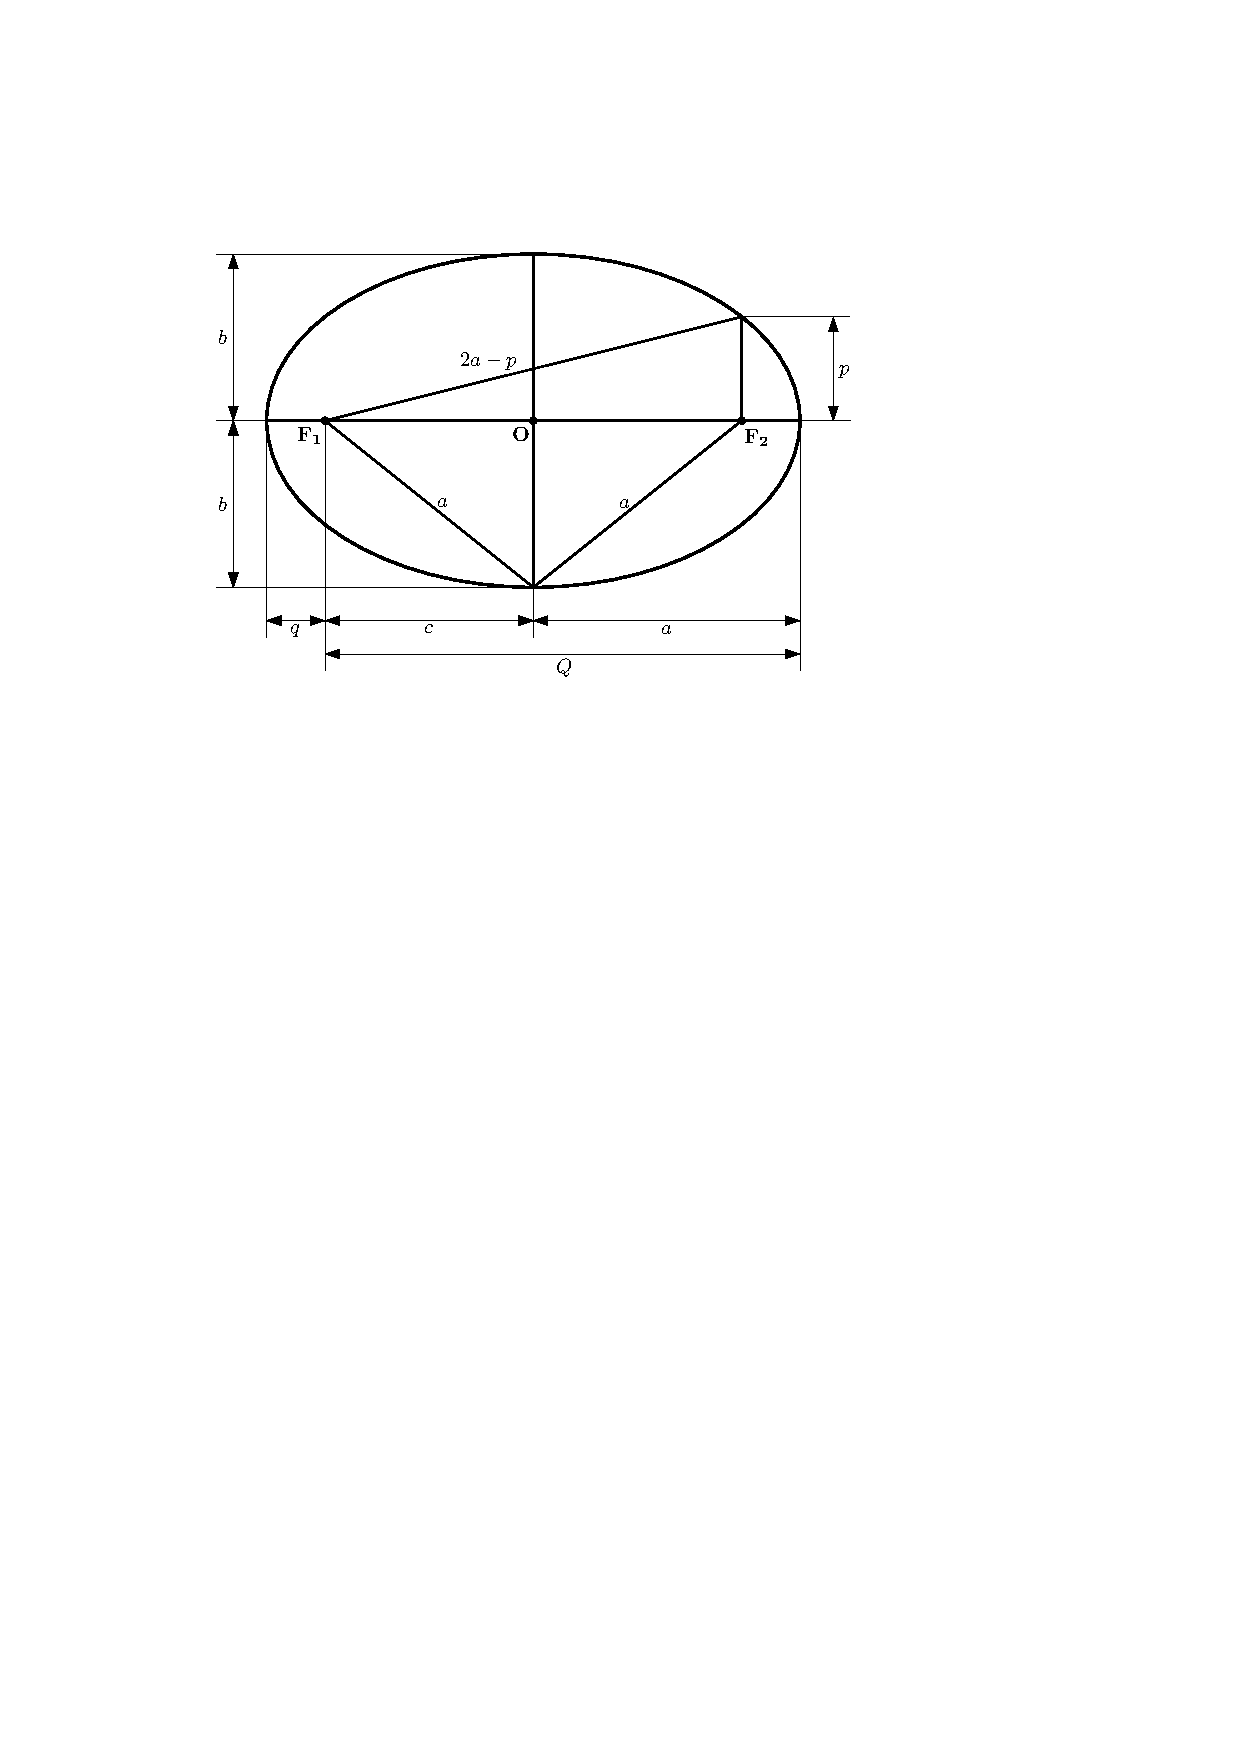
\includegraphics[width = .97\tw]{Ellips}
		\captionof{figure}{Эллипс}
		\label{pic:ellipse}
	\end{flushright}
\end{minipage}

\change{
Рассмотрим крайнюю левую и крайнюю правую точки эллипса на Рис.~\ref{pic:ellipse}, назовем их $A$ и $B$ соответственно, тогда сумма расстояний $l$ от каждой из них до фокусов $F_1$ и $F_2$ равна:
\begin{equation*}
	AF_1 + AO + OF_2 = AF_1 + a + c = l = BF_2 + BO + OF_1 = BF_2 + a + c.
\end{equation*}
Откуда следует, что $A F_1 = B F_2$. Легко видеть, что $AB = 2a$, значит $l = AF_1 + AO + OF_2 = AO + OF_2 + F_2B = 2a$. Получается, сумма расстояний до фокусов от любой точки эллипса равна его удвоенной большой полуоси.
}

\change{
В силу равенства прямоугольных треугольников $\triangle F1 O C$ и $\triangle F_2 O C$ равны их гипотенузы $F_1C$ и $F_2C$, причем $F_1C= F_2C = l/2 = a$. Отсюда получается одно из основных соотношений в эллипсе:
}
\begin{equation}
	b^2 + c^2 = a^2.
\end{equation}
\term{Эксцентриситет} ($e$)~--- числовая
характеристика, показывающая степень отклонения конического сечения от окружности. Для эллипса $e$ лежит в интервале $(0, \, 1)$ и
определяется формулой
\begin{equation}
	e = \frac{c}{a}.
\end{equation}

\term{Апоцентр}~--- наиболее удаленная
от заданного фокуса точка эллипса. Из определения эллипса
вытекает соотношение для расстояния от фокуса до
апоцентра ($Q$):
\begin{equation}
	Q = a (1 + e).
\end{equation}

\term{Перицентр}~--- ближайшая
точка эллипса к заданному фокусу. Из определения эллипса
вытекает соотношение для расстояния от фокуса до
перицетра ($q$):
\begin{equation}
	q = a (1 - e).
\end{equation}

\term{Фокальный параметр}~($p$)~--- длина перпендикуляра,
проведенного из фокуса до точки пересечения с эллипсом.
Из теоремы Пифагора и определения эллипса следует
нижеприведенная формула для расчета его длины:
\begin{equation}
	p=\frac{b^2}{a}=a(1-e^2)=b\sqrt{1-e^2}.
\end{equation}

\term{Площадь эллипса} ($S$) --- площадь части
плоскости, ограниченной эллипсом, равна
\begin{equation}
	S = \pi ab = \pi a^2 \sqrt{1-e^2}.
\end{equation}

%Радиус кривизны дуги эллипса в зависимости от расстояния
%$x$ от фокуса:
%\begin{equation}
%R=\frac{(2ax-x^2)^{3/2}}{ab}
%\end{equation}
%\begin{center}
%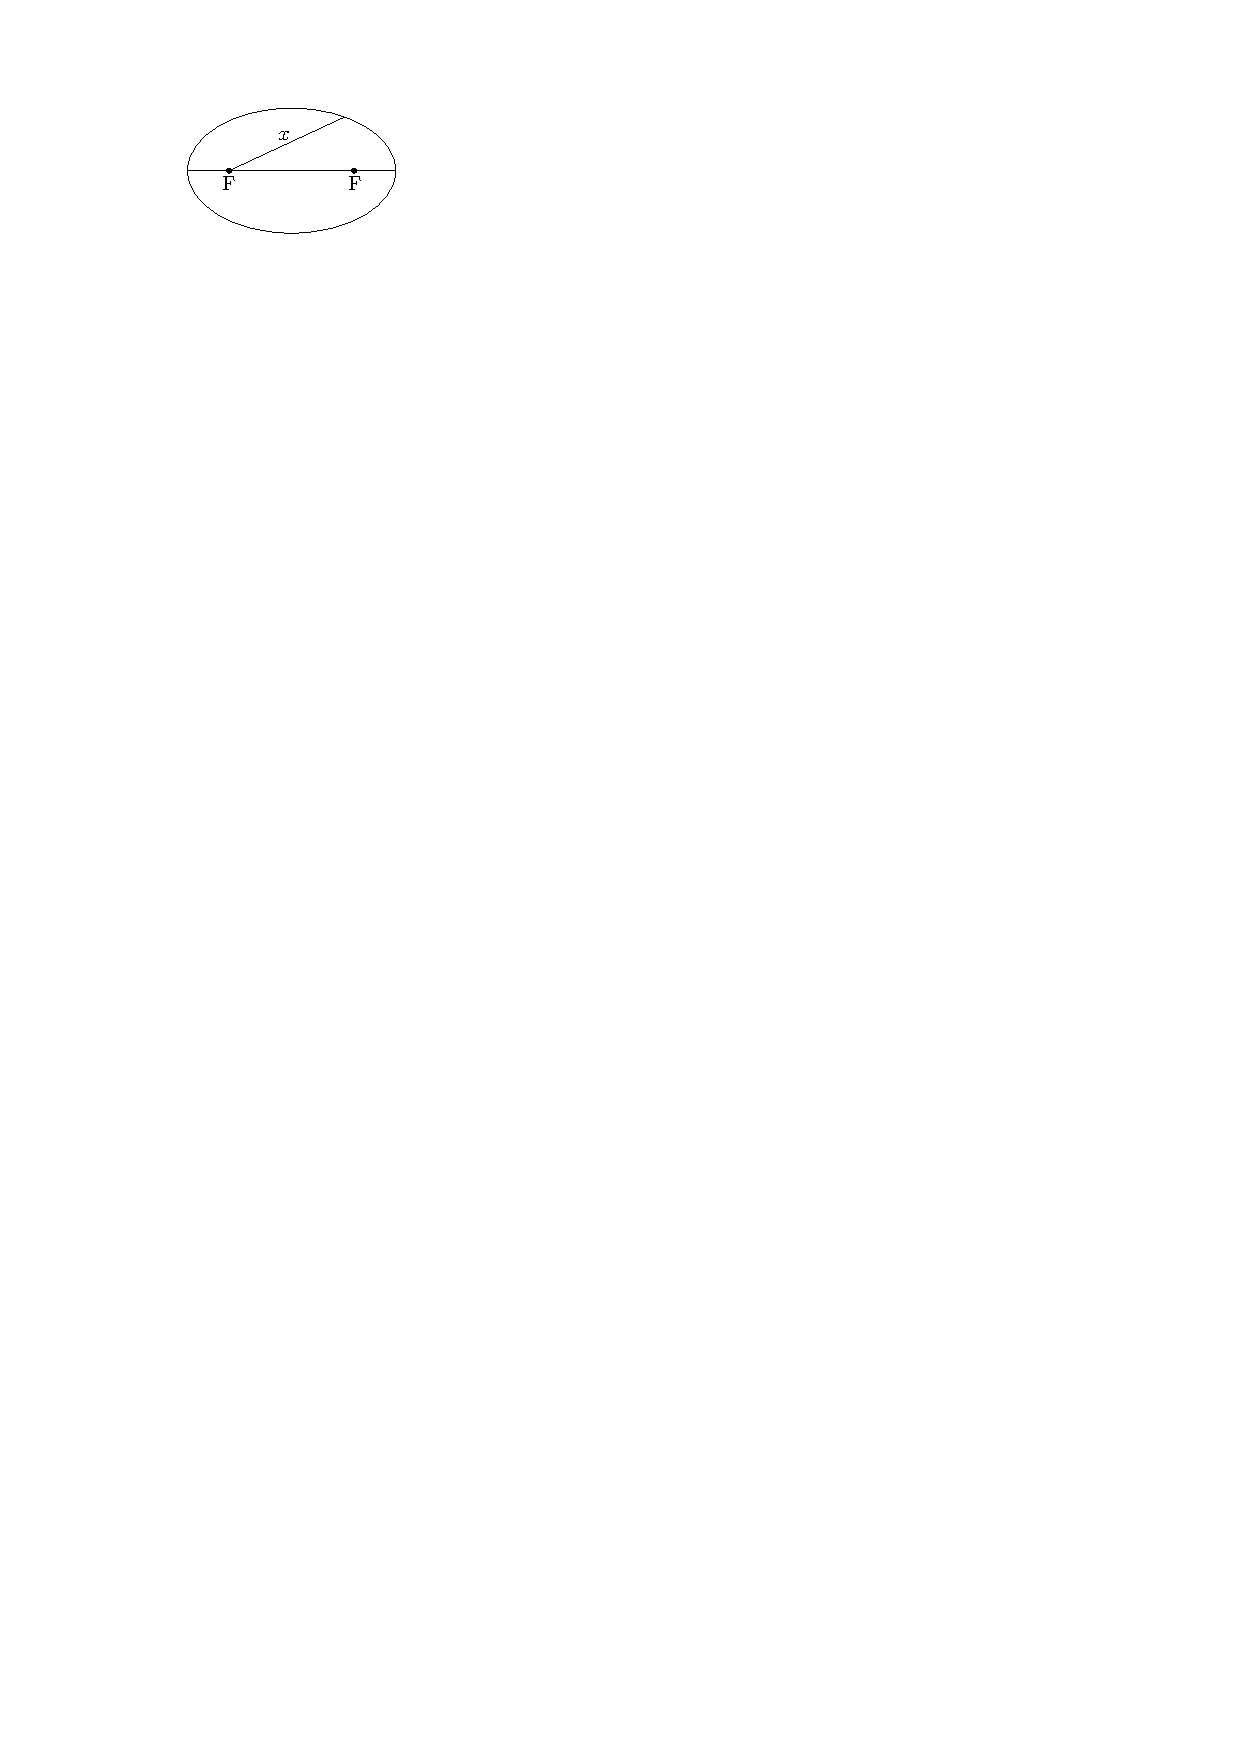
\includegraphics[width = 0.3\textwidth]{rad-curv}
%\begin{figure}[!h]
%\caption{К вычислению радиуса кривизны эллипса}
%\end{figure}
%\end{center}

{\itshape Уравнение эллипса} в декартовых координатах
представляет собой уравнение замкнутой кривой второго
порядка, канонический вид которого:
\begin{equation}
	\frac{x^2}{a^2}+\frac{y^2}{b^2}=1.
\end{equation}

Его можно представить параметрическом виде:
\begin{equation}
	\left\{
	\begin{aligned}[lcl]
		&x=a\cos t,\\
		&y=b\sin t;\\
	\end{aligned}
	\right. \quad\quad t \in [0, \, 2\pi).
\end{equation}
В полярных координатах уравнение принимает следующий вид:
\begin{equation}
	r=\frac{p}{1\pm e \cos \varphi},
	\label{eq:ellipse-pol-eq}
\end{equation}
\begin{wrapfigure}[11]{l}{0.5\tw}
	\centering
	\vspace{-.7pc}
	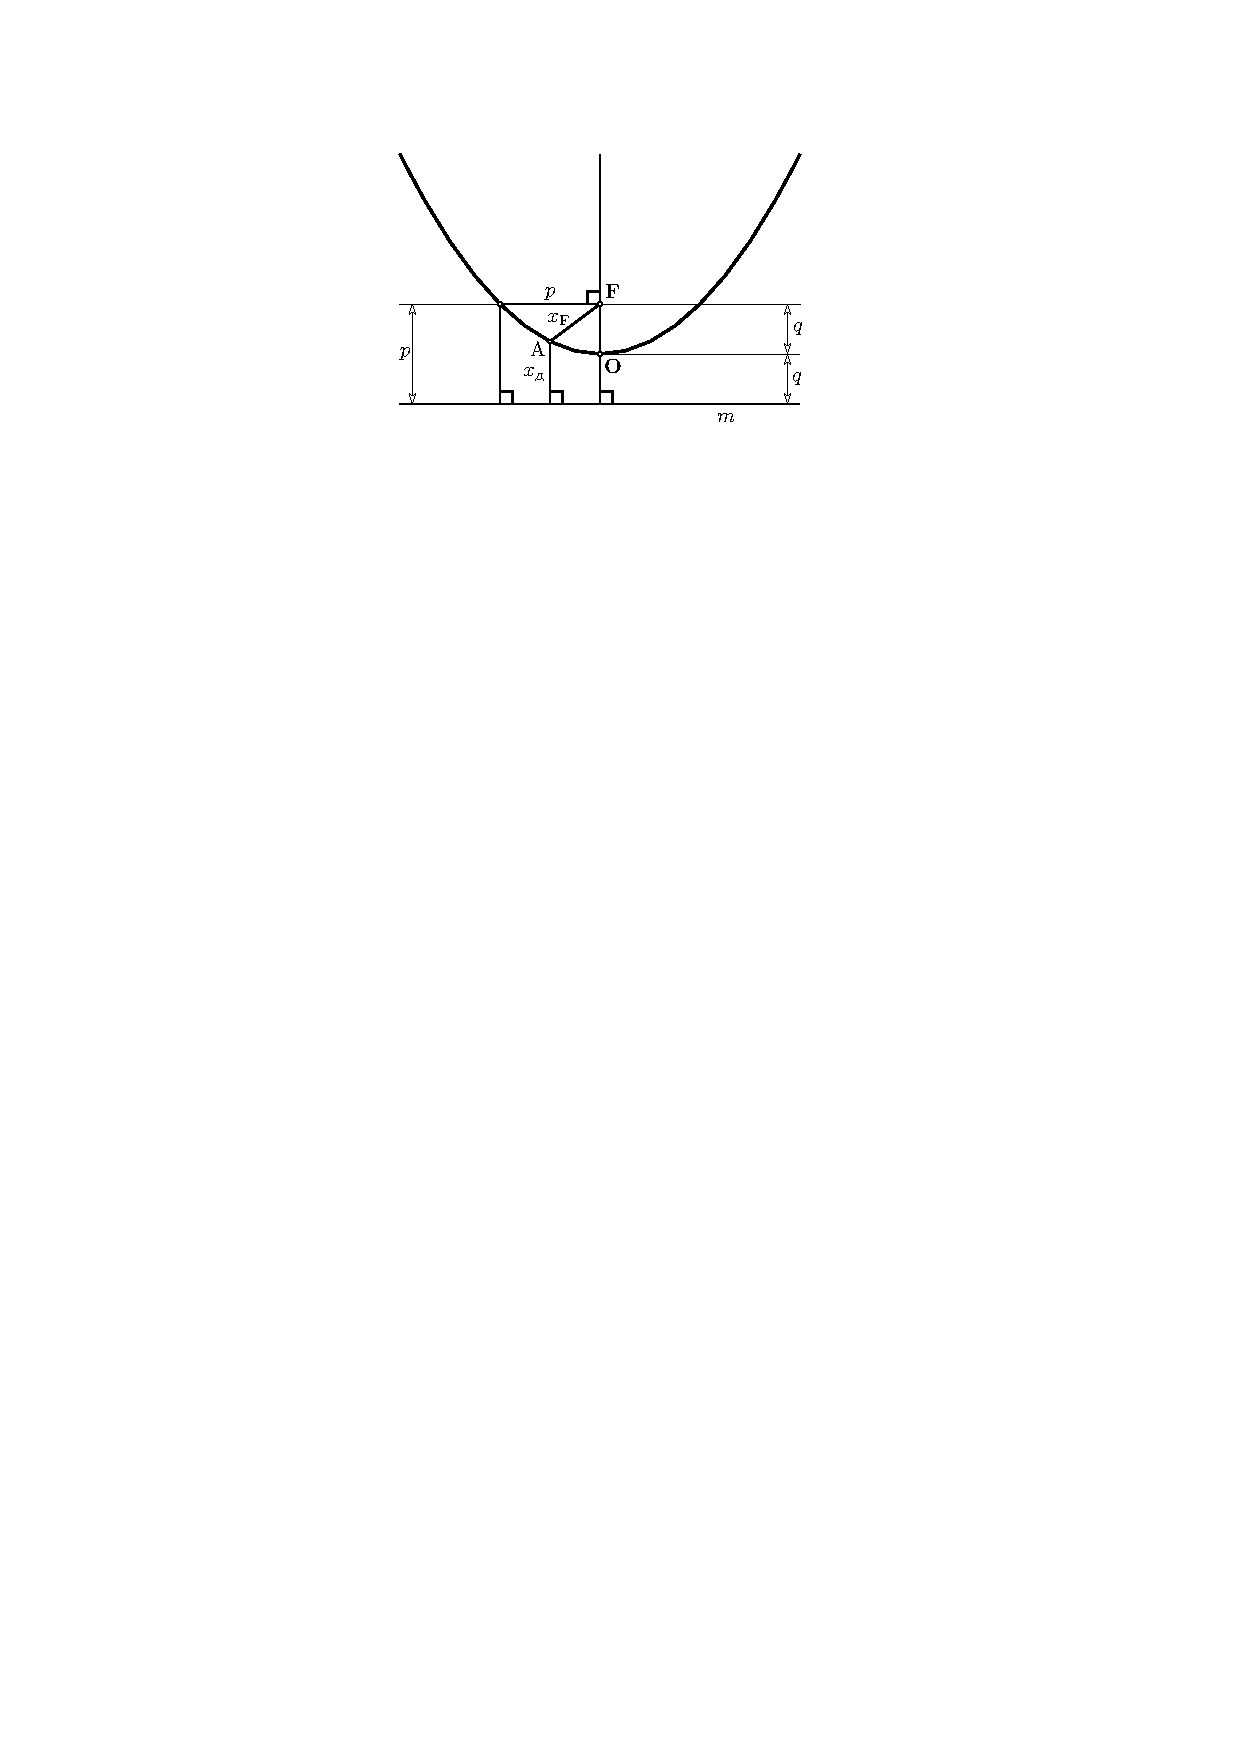
\includegraphics[width = 0.5\tw]{Parabola}
	\captionof{figure}{Парабола \label{pic:the-pic}}
\end{wrapfigure}
где $\varphi$ --- \term{истинная аномалия} --- угол
{\slshape перицентр -- фокус -- заданная точка},
отсчитываемый в сторону движения по эллипсу. При
знаке плюс перед $e$ второй фокус эллипса будет
находится в точке $(0, \, 2c)$, а при минус --- в
точке $(\pi, \, 2c)$.

Кроме этого, эллипс обладает важным {\itshape оптическим
свойством}, которое можно сформулировать так: свет от источника в одном из фокусов,
отражается эллипсом так, что отражённые лучи пересекаются
во втором фокусе или, что тоже самое, касательная к эллипсу в заданной точке образует с фокальными радиусами в данной точке равные острые углы.

